%==============================================================================
%  PhD Research Presentation Series — June 2026
%  Paper 1: European Fixed Income Arbitrages
%  Author: Alessio Ottaviani  |  Supervisor: Prof. Riccardo Rebonato (EDHEC)
%
%  BLOCK 1 (slides 1-9):  Opening + Strategy Setup
%==============================================================================

\documentclass[aspectratio=169,11pt]{beamer}

%------------------------------------------------------------------------------
%  THEME
%------------------------------------------------------------------------------
\mode<presentation>{
  \usetheme{CambridgeUS}
  \usecolortheme{default}
}

%------------------------------------------------------------------------------
%  PACKAGES
%------------------------------------------------------------------------------
\usepackage{graphicx}
\usepackage{booktabs}
\usepackage{amsmath, amssymb, amsthm}
\usepackage{array}
\usepackage{multirow}
\usepackage{tikz}
\usetikzlibrary{shapes, arrows, positioning, fit, backgrounds}
\usepackage{threeparttable}
\usepackage{hyperref}
\usepackage{lmodern}
\usepackage{ragged2e}
\usepackage{xltabular}
\usepackage{setspace}
\usepackage{xcolor}
\usepackage{colortbl}

% Citations: natbib + bibtex (same as paper, compatible with paper1_refs.bib)
\usepackage[authoryear,round]{natbib}
\bibliographystyle{plainnat}

%------------------------------------------------------------------------------
%  COLOURS — coherent with paper highlights
%------------------------------------------------------------------------------
\definecolor{edhecred}{RGB}{170,30,45}
\definecolor{accentblue}{RGB}{30,80,150}
\definecolor{softgrey}{RGB}{100,100,100}
\definecolor{myblue}{RGB}{0, 51, 102}
\definecolor{myred}{RGB}{153, 0, 0}
\definecolor{mygreen}{RGB}{0, 102, 51}
\definecolor{mygold}{RGB}{204, 153, 0}
\definecolor{lightgray}{RGB}{240, 240, 240}
\newcommand{\hlt}[1]{\textcolor{edhecred}{\textbf{#1}}}     % main highlight
\newcommand{\hltb}[1]{\textcolor{accentblue}{\textbf{#1}}}  % secondary highlight

%------------------------------------------------------------------------------
%  LAYOUT — narrow banner, tight margins
%------------------------------------------------------------------------------
\setbeamerfont{frametitle}{size=\normalsize}
\makeatletter
\setbeamertemplate{frametitle}{%
  \nointerlineskip%
  \vskip-4pt%
  \begin{beamercolorbox}[wd=\paperwidth,ht=2.3ex,dp=0.8ex,center]{frametitle}%
    \usebeamerfont{frametitle}\insertframetitle
  \end{beamercolorbox}%
  \vskip0pt%
}
\makeatother

% Tight horizontal margins
\setbeamersize{text margin left=3mm,text margin right=3mm}

% Footer: page number + section
\setbeamertemplate{footline}{%
  \leavevmode%
  \hbox{%
    \begin{beamercolorbox}[wd=.5\paperwidth,ht=2.5ex,dp=1ex,leftskip=2ex]{author in head/foot}%
      \usebeamerfont{author in head/foot}\insertshortauthor\hspace{0.5em}--\hspace{0.5em}\insertshorttitle
    \end{beamercolorbox}%
    \begin{beamercolorbox}[wd=.5\paperwidth,ht=2.5ex,dp=1ex,rightskip=2ex,right]{title in head/foot}%
      \usebeamerfont{title in head/foot}\insertsection\hspace{1em}\insertframenumber/\inserttotalframenumber
    \end{beamercolorbox}%
  }%
  \vskip0pt%
}

% Remove navigation symbols
\setbeamertemplate{navigation symbols}{}

% Itemize style
\setbeamertemplate{itemize items}[circle]
\setbeamercolor{itemize item}{fg=edhecred}
\setbeamercolor{itemize subitem}{fg=accentblue}

% Block templates: rounded, with subtle shadow
\setbeamertemplate{blocks}[rounded][shadow=false]

% Custom block colors (visible boxes)
\setbeamercolor{block title}{fg=white,bg=accentblue}
\setbeamercolor{block body}{fg=black,bg=accentblue!8}

\setbeamercolor{block title alerted}{fg=white,bg=edhecred}
\setbeamercolor{block body alerted}{fg=black,bg=edhecred!8}

\setbeamercolor{block title example}{fg=white,bg=mygreen}
\setbeamercolor{block body example}{fg=black,bg=mygreen!8}

% Graphics path — covers paper repo layouts
% Graphics path — slides live in C:\Users\aless\Desktop\THESIS\slides\
% results\ folder lives in        C:\Users\aless\Desktop\THESIS\results\
% So from slides folder, paper figures are at ../results/figures/ etc.
\graphicspath{%
  {./}%
  {figures/}%
  {../results/figures/}%
  {../results/figures/strategies/}%
  {../results/figures/pca/}%
  {../results/figures/aen/}%
  {../results/rq3_duffie/figures/}%
}

% Tablepath: location of \input{...} tables
\newcommand{\tablepath}{../results/tables}

%------------------------------------------------------------------------------
%  TITLE METADATA
%------------------------------------------------------------------------------
\title[European FI Arbitrages]{Exploring Excess Return Generation through \\
  European Fixed Income Arbitrages}
\subtitle{BTP Italia, the CDS--Bond Basis, and the iTraxx Index Skew}

\author[A.\ Ottaviani]{Alessio Ottaviani}
\institute[EDHEC]{
  EDHEC Business School \\[0.15cm]
  \textit{Supervisor:} Prof.\ Riccardo Rebonato
}
\date{PhD Research Presentation Series \\ June 2026}

%==============================================================================
%  DOCUMENT
%==============================================================================
\begin{document}

%==============================================================================
%  BLOCK 1 — OPENING  (slides 1-4, ~4 minutes)
%==============================================================================

%------------------------------------------------------------------------------
% SLIDE 1 — Title page
%------------------------------------------------------------------------------
\begin{frame}[plain]
  \titlepage
\end{frame}

%------------------------------------------------------------------------------
% SLIDE 2 — Motivation: The Steamroller Question
%------------------------------------------------------------------------------
\section{Motivation}

\begin{frame}[t]{Motivation: The Steamroller Question}
\vspace{0.2cm}

\textbf{\citet{duarte2007risk} pose the question that motivates this paper:}

\vspace{0.35cm}
\begin{quote}
  \itshape
  Do fixed-income arbitrage strategies earn genuine alpha, or are their returns
  simply compensation for systematic risk\,---\,``picking up nickels in front
  of a steamroller''?
\end{quote}

\vspace{0.35cm}

\textbf{Their answer:} the more complex strategies generate \hlt{significant alpha}
that survives a 10-factor benchmark in U.S.\ markets.

\vspace{0.5cm}

\textbf{Open questions that motivate this paper:}
\begin{itemize}\itemsep=0.2cm
  \item Does the result generalise to \hltb{European} fixed-income markets?
  \item Does it survive a \hltb{much more demanding} battery of factor controls?
  \item And\,---\,perhaps above all\,---\,\hltb{why does the alpha persist}?
\end{itemize}

\end{frame}

%------------------------------------------------------------------------------
% SLIDE 3 — Research Questions
%------------------------------------------------------------------------------
\begin{frame}[t]{Research Questions}
\vspace{0.15cm}

\small

\begin{block}{\normalsize RQ1.\ \ \emph{Does alpha exist?}}
Do three European fixed-income arbitrage strategies\,---\,the BTP Italia
inflation-linked basis, the corporate CDS--Bond basis, and the iTraxx
index skew\,---\,generate excess returns that survive standard
benchmark factor models?
\hfill\textcolor{softgrey}{\footnotesize $\rightarrow$ Section 3}
\end{block}

\vspace{0.15cm}

\begin{block}{\normalsize RQ2.\ \ \emph{Does alpha survive aggressive risk adjustment\,---\,and is it state-dependent?}}
Does the alpha survive when the candidate factor universe is enlarged
to \textbf{85} controls and selected by data-driven methods (rolling PCA;
Adaptive Elastic Net with stability selection)?
And: does the residual alpha vary systematically with intermediary funding stress?
\hfill\textcolor{softgrey}{\footnotesize $\rightarrow$ Section 4}
\end{block}

\vspace{0.15cm}

\begin{block}{\normalsize RQ3.\ \ \emph{Why does alpha persist?}}
Are the three mispricings linked to one another, and is the
co-movement consistent with the slow-moving capital framework
of \citet{duffie2010presidential}?
\hfill\textcolor{softgrey}{\footnotesize $\rightarrow$ Section 5}
\end{block}

\end{frame}

%------------------------------------------------------------------------------
% SLIDE 4 — What's New: Four Contributions
%------------------------------------------------------------------------------
\begin{frame}[t]{What's New: Four Contributions}
\small
\vspace{0.15cm}

\begin{enumerate}\itemsep=0.30cm

  \item \hlt{Deterministic payoff at maturity.}\\[0.05cm]
  Each strategy converges with certainty if held to maturity\,---\,unlike
  Duarte's swap spreads, yield-curve trades, mortgage hedging, volatility selling
  or capital-structure trades, whose payoffs are model-dependent.

  \item \hlt{A progressive battery of increasingly demanding factor controls.}\\[0.05cm]
  Three classical benchmarks (Duarte 2007; Brooks 2020; Fung--Hsieh 2004)
  $\to$ rolling PCA on 85 candidate factors $\to$ Adaptive Elastic Net with
  stability selection $\to$ Ferson--Schadt conditional alpha.

  \item \hlt{Joint cross-strategy test of Duffie (2010).}\\[0.05cm]
  Five testable predictions (P1--P5) of slow-moving capital, tested
  \emph{jointly}\,---\,with a natural experiment built into the design:
  CDS--Bond and iTraxx (institutional) vs.\ BTP Italia (retail).

  \item \hlt{The post-crisis regulatory capital channel.}\\[0.05cm]
  Basel III has \emph{permanently} raised intermediary balance-sheet costs
  (Boyarchenko et al.\ 2016): persistent alpha is the \emph{equilibrium}, not
  a transient anomaly.

\end{enumerate}
\end{frame}

%==============================================================================
%  BLOCK 2 — STRATEGIES & DATA  (slides 5-9, ~5 minutes)
%==============================================================================

%------------------------------------------------------------------------------
% SLIDE 5 — The Three Strategies (Synoptic)
%------------------------------------------------------------------------------
\section{Strategies and Data}

\begin{frame}[t]{Three European Fixed-Income Arbitrages}
\small
\vspace{0.10cm}

\begin{columns}[t]
\column{0.32\textwidth}
\begin{block}{\textbf{BTP Italia}\\ \footnotesize Inflation-Linked Basis}
\scriptsize
\textbf{Trade:} ASW BTP Italia vs nominal BTP \\[3pt]
\textbf{Sample:} Mar 2012 -- May 2025 (260 trades) \\[3pt]
\textbf{Bond holders:} \\
\textcolor{myred}{\textbf{Retail-dominated}} (loyalty bonus) \\[3pt]
\textbf{New:} no prior academic study; eliminates ballooning risk
\end{block}

\column{0.32\textwidth}
\begin{block}{\textbf{CDS--Bond Basis}\\ \footnotesize Negative Basis Trade}
\scriptsize
\textbf{Trade:} Long bond + Long CDS protection \\[3pt]
\textbf{Sample:} Sep 2008 -- May 2025 (931 trades) \\[3pt]
\textbf{Bond holders:} \\
\textcolor{mygreen}{\textbf{Institutional}} (dealers, HFs) \\[3pt]
\textbf{New:} Euro counterpart of \citet{bai2019cds}
\end{block}

\column{0.32\textwidth}
\begin{block}{\textbf{iTraxx Combined}\\ \footnotesize CDS Index Skew}
\scriptsize
\textbf{Trade:} Index vs duration-weighted single names \\[3pt]
\textbf{Sample:} Jun 2004 -- May 2025 (206 trades) \\[3pt]
\textbf{Bond holders:} \\
\textcolor{mygreen}{\textbf{Institutional}} (dealers, HFs) \\[3pt]
\textbf{New:} 4 EU sub-indices; not previously studied jointly
\end{block}
\end{columns}

\vspace{0.45cm}

\centering
\hltb{Two clusters by bond-holder base $\Rightarrow$ natural experiment for Duffie\,(2010).}\\[0.15cm]
{\footnotesize \emph{Arbitrageurs} are always institutional (asset-swap, repo, CDS access).
``Bond holders'' refers to who \emph{holds the underlying bonds}\,---\,the natural counterparty
of the arbitrage trade.}

\end{frame}

%------------------------------------------------------------------------------
% SLIDE 6 — BTP Italia: Why It's Different from TIPS
%------------------------------------------------------------------------------
\begin{frame}[t]{BTP Italia: Why It's Different from TIPS}
\footnotesize
\vspace{0.10cm}

\textbf{First instrument-level study of the BTP Italia inflation-linked basis in the academic literature.}
Two structural features distinguish it from \citet{fleckenstein2014tips}'s TIPS--Treasury basis.

\vspace{0.30cm}

\begin{columns}[t]
\column{0.50\textwidth}
\begin{exampleblock}{No ballooning risk}
\scriptsize
Conventional ILBs accumulate inflation in principal: a TIPS with $I_t=1.25$ has notional $125$. \\[4pt]
In default, recovery applied to the inflation-adjusted principal $\rightarrow$ investor loses cumulated revaluation. \\[4pt]
\textbf{BTP Italia} pays revaluation each coupon, redeems at par. Notional exposed to credit risk $= 100$ throughout life of bond. \\[4pt]
$\rightarrow$ \emph{Less risk, yet positive basis.}
\end{exampleblock}

\column{0.50\textwidth}
\begin{exampleblock}{Retail bond holders $\rightarrow$ segmentation}
\scriptsize
Two-phase placement: retail-only first phase + \textit{premio fedelt\`a} (loyalty bonus). Households hold to maturity. \\[4pt]
\textcolor{myred}{\textbf{Key:}} retail does not face margin calls or balance-sheet constraints, and \emph{cannot themselves} run the BTP Italia / nominal BTP arbitrage (ASW + repo + inflation-swap infrastructure required). \\[4pt]
$\rightarrow$ \emph{Preferred-habitat} bond holder base \citep{vayanos2021preferred}: the natural counterparty does not unwind in stress, structurally insulated from the institutional fire-sale dynamics that close the U.S.\ TIPS basis.
\end{exampleblock}
\end{columns}

\end{frame}

%------------------------------------------------------------------------------
% SLIDE 7 — CDS-Bond Basis: Definition & Negative Basis Trade
%------------------------------------------------------------------------------
\begin{frame}[t]{CDS--Bond Basis: The Negative Basis Trade}
\small

\textbf{Definition.}\hfill {\small For issuer $i$ at date $t$:}
\[
  \text{Basis}_{i,t} \;=\; \text{CDS spread}_{i,t} \;-\; \text{z-spread}_{i,t}
\]
where the z-spread is the constant additive spread that, on the bootstrapped
EUR zero-coupon swap curve, equates the discounted bond cash flows to its
market price.

\vspace{0.30cm}

\textbf{Trade construction.}
\begin{itemize}\itemsep=0.10cm
  \item Negative basis $\Rightarrow$ CDS protection cheaper than the credit spread
        embedded in the bond price.
  \item \emph{Negative basis trade only:} buy the bond (earn z-spread)
        + buy CDS protection (pay CDS premium) $\to$ \hlt{positive carry locked in
        until convergence or maturity}.
  \item \emph{Why not the reverse trade?} Short bond requires sourcing it via
        reverse repo $\to$ recall risk during stress \citep{bai2019cds}.
  \item \hltb{In default:} bond recovers $RR$, CDS pays $100-RR$
        $\Rightarrow$ combined position returns par regardless of recovery
        (provided CDS maturity $\geq$ bond residual life).
  \item \emph{Universe:} single names in the on-the-run iTraxx Europe Main 5Y.\
        Liquidity filter $+$ IG quality control. All CDS centrally cleared
        (LCH / ICE).
\end{itemize}

\end{frame}

%------------------------------------------------------------------------------
% SLIDE 8 — iTraxx Combined: The Skew Across Sub-Indices
%------------------------------------------------------------------------------
\begin{frame}[t]{iTraxx Combined: The CDS Index Skew}
\small

\textbf{Definition.}\hfill {\small Skew of an iTraxx index relative to its constituents:}
\[
  \text{Skew}_t \;=\; S_t^{\text{index}} \;-\; \sum_{i=1}^{N} w_{i,t}\, S_{i,t}^{\text{single}}
\]
where the duration weights $w_{i,t}$ ensure the replicating portfolio matches
the aggregate credit risk sensitivity of the index.

\vspace{0.30cm}

\textbf{Sources of the skew.}\ \ Liquidity differentials between index and
single names; hedging demand for portfolio credit protection; dealer inventory
costs; replication operational cost.

\vspace{0.30cm}

\textbf{Strategy design.}
\begin{itemize}\itemsep=0.07cm
  \item \emph{Four sub-indices}: Main, Senior Financials, Subordinated
        Financials, Crossover\,---\,only \hlt{on-the-run} series at entry.
  \item Entry thresholds calibrated to each sub-index's historical volatility
        $\Rightarrow$ wider thresholds for Crossover than for Main.
  \item Most mispriced sub-index (absolute basis) traded at each decision date;
        both index and single-name CDS centrally cleared.
\end{itemize}

\end{frame}

%------------------------------------------------------------------------------
% SLIDE 9 — Trade Construction & Index Aggregation
%------------------------------------------------------------------------------
\begin{frame}[t]{Trade Construction \& Index Aggregation}
\small

\textbf{Following \citet{duarte2007risk}.} Each individual trade is treated as
a separate fictional fund (own entry/exit/return stream); the strategy
index on any day is the weighted average of the returns of the funds active
on that day.

\vspace{0.20cm}

\textbf{Two weighting schemes:}
\begin{columns}[T]
  \begin{column}{0.46\textwidth}
    \emph{Equal-Weighted (\citealp{duarte2007risk})}
    \[
      r_t^{\text{EW}} \;=\; \frac{1}{K_t}\sum_{k=1}^{K_t} r_{k,t}
    \]
  \end{column}
  \begin{column}{0.54\textwidth}
    \emph{Signal-Weighted (\citealp{rebonato2021convexity})}
    \[
      r_t^{\text{SW}} \;=\; \sum_{k=1}^{K_t}
        \frac{|b_{k,0} - \theta_{t_k}|}
             {\sum_{j=1}^{K_t}|b_{j,0} - \theta_{t_j}|} \, r_{k,t}
    \]
  \end{column}
\end{columns}

\vspace{0.05cm}
{\footnotesize $b_{k,0}$: basis at entry of trade $k$;\
$\theta_{t_k}$: expanding-window historical equilibrium up to entry.\
Weight $\propto$ distance from equilibrium $\to$ richer dislocation, larger allocation.}

\vspace{0.20cm}

\textbf{Implementation choices.}
\begin{itemize}\itemsep=0.06cm
  \item \hlt{SW dominates EW} on Sharpe and MPPM for all three strategies
        $\to$ SW baseline; EW in appendix confirms robustness.
  \item Three-regime classification on iTraxx Main 5Y\,---\,
        \emph{LOW} ($<60$\,bps), \emph{MID} (60--100\,bps),
        \emph{HIGH} ($>100$\,bps)\,---\,drives \hltb{regime-dependent
        transaction costs} (entry/exit fees proportional to DV01).
\end{itemize}

\end{frame}

%==============================================================================
%  BLOCK 3 — PERFORMANCE  (slides 10-13, ~4 minutes)
%==============================================================================

%------------------------------------------------------------------------------
% SLIDE 10 — Summary Statistics
%------------------------------------------------------------------------------
\section{Performance}

\begin{frame}[t]{Strategy Performance: Summary Statistics}
\centering
\small
\vspace{0.10cm}

\textit{Annualised, daily data, net of regime-dependent transaction costs.}

\vspace{0.20cm}
\renewcommand{\arraystretch}{1.20}
\setlength{\tabcolsep}{8pt}

\begin{tabular}{lccc}
\toprule
 & \textit{BTP Italia} & \textit{CDS--Bond Basis} & \textit{iTraxx Combined} \\
\midrule
Sample             & Mar\,2012 -- May\,2025 & Sep\,2008 -- May\,2025 & Jun\,2004 -- May\,2025 \\
Mean return (\%)   & 1.67  & \hlt{5.37}  & 1.96  \\
Volatility (\%)    & 2.34  & 3.15  & 2.59  \\
\hlt{Sharpe ratio} & 0.71  & \hlt{1.71}  & 0.76  \\
Skewness           & +0.43 & +0.60 & \hlt{+2.81} \\
Max drawdown (\%)  & 3.0   & 4.4   & 2.5   \\
Basis $\rho_1$ (daily) & 0.98 & 0.92 & 0.87  \\
\bottomrule
\end{tabular}

\vspace{0.30cm}

\begin{itemize}\itemsep=0.07cm\footnotesize
  \item Sharpe ratios from \hltb{0.71} (BTP Italia) to \hltb{1.71}
        (CDS--Bond)\,---\,economically large, statistically significant.
  \item \emph{Positive skewness} for all three (max $+2.81$ for iTraxx)
        $\Rightarrow$ cuts against ``picking up nickels in front of a steamroller''.
  \item Persistence $\rho_1 \in [0.87,\,0.98]$ on the underlying basis
        $\Rightarrow$ slow-moving capital signature \citep{duffie2010presidential}.
\end{itemize}

\end{frame}

%------------------------------------------------------------------------------
% SLIDE 11 — Cumulative Returns & Drawdowns
%------------------------------------------------------------------------------
\begin{frame}[t]{Cumulative Returns and Drawdowns}
\vspace{-0.05cm}
\centering

% Figure 11 — equity curves combined
\includegraphics[width=0.85\textwidth,keepaspectratio]{equity_curves_combined.pdf}

\vspace{0.30cm}

\begin{itemize}\itemsep=0.08cm\small
  \item Smooth, near-monotone equity curves for all three strategies.
  \item \hlt{Max drawdowns: 4.4\% / 3.0\% / 2.5\%}\,---\,all recovered within months.
  \item Deepest drawdowns cluster in 2008--09 (CDS--Bond), 2011--12 sovereign
        crisis (BTP Italia), and 2020 COVID\,---\,each is a known
        intermediary-stress episode, not idiosyncratic noise.
\end{itemize}

\end{frame}

%------------------------------------------------------------------------------
% SLIDE 12 — Manipulation-Proof Performance (MPPM)
%------------------------------------------------------------------------------
\begin{frame}[t]{Manipulation-Proof Performance \citep{goetzmann2007portfolio}}
\centering
\small
\vspace{0.10cm}

\textit{MPPM (\% p.a.) for risk-aversion parameters $\rho \in \{2,3,4\}$. SW index, monthly.}

\vspace{0.20cm}
\renewcommand{\arraystretch}{1.25}
\setlength{\tabcolsep}{12pt}

\begin{tabular}{lccc}
\toprule
 & $\rho=2$ & $\rho=3$ & $\rho=4$ \\
\midrule
\textit{BTP Italia}      & 1.56 & 1.55 & 1.54 \\
\textit{CDS--Bond Basis} & \hlt{5.06} & \hlt{5.01} & \hlt{4.97} \\
\textit{iTraxx Combined} & 1.83 & 1.82 & 1.80 \\
\bottomrule
\end{tabular}

\vspace{0.50cm}

\begin{itemize}\itemsep=0.10cm\small
  \item MPPM is the unique measure that cannot be manipulated by dynamic
        rules, leverage, or information-free trading\,---\,the right
        benchmark for strategies with state-dependent entry/exit.
  \item \hlt{Near-invariance to $\rho$}: a $\rho=4$ investor evaluates these
        strategies essentially the same way as a $\rho=2$ investor.
        Read with positive skewness $\Rightarrow$ documented Sharpe
        ratios are \hltb{not compensation for unobserved tail risk}.
\end{itemize}

\end{frame}

%------------------------------------------------------------------------------
% SLIDE 13 — Volatility-Managed Portfolios (Moreira-Muir)
%------------------------------------------------------------------------------
\begin{frame}[t]{Volatility-Managed Portfolios \citep{moreira2017volatility}}
\centering
\small
\vspace{0.10cm}

\[
  f^{\sigma}_{t+1} \;=\; \frac{c}{\hat{\sigma}^2_t}\, f_{t+1}
  \qquad\Longrightarrow\qquad
  r^{VM}_{t+1} \;=\; \alpha + \beta\, r_{t+1} + \varepsilon_{t+1}
\]

{\footnotesize Significant $\alpha$ $\Leftrightarrow$ time-varying $\mu_t/\sigma_t^2$.}

\vspace{0.30cm}

\renewcommand{\arraystretch}{1.20}
\setlength{\tabcolsep}{10pt}
\begin{tabular}{lccc}
\toprule
 & \textit{BTP Italia} & \textit{CDS--Bond Basis} & \textit{iTraxx Combined} \\
\midrule
Managed $\alpha$ (\% p.a.) & $-0.22$ & \hlt{$+1.68^{**}$} & $-0.16$ \\
Significance               & ns      & sig.\ at 5\%      & ns      \\
\bottomrule
\end{tabular}

\vspace{0.45cm}

\begin{itemize}\itemsep=0.10cm\small
  \item \hlt{CDS--Bond}: significant managed alpha
        $\Rightarrow$ time-varying \emph{funding-liquidity} mechanism
        (capital available when vol low, withdraws when vol high).
  \item BTP Italia, iTraxx: stable risk-return trade-off, vol overlay
        cannot exploit.
  \item \hltb{Foreshadow:} the time-variation here is strategy-specific, but
        regime-dependent alpha (Section 3.3) shows it
        \emph{generalises} to all three strategies once we control for benchmark
        factor exposures.
\end{itemize}

\end{frame}

%==============================================================================
%  BLOCK 4 — BENCHMARK FACTOR MODELS  (slides 14-18, ~5 minutes)
%==============================================================================

%------------------------------------------------------------------------------
% SLIDE 14 — Three Benchmark Frameworks: Setup
%------------------------------------------------------------------------------
\section{Benchmark Factor Models}

\begin{frame}[t]{Three Benchmark Frameworks}
\small

\textbf{We test the alpha against the three canonical benchmarks of the FI-arbitrage
and active FI literature.}

\vspace{0.30cm}

\begin{itemize}\itemsep=0.20cm

  \item \hlt{\citet{duarte2007risk}} \emph{(RFS)} \,---\, the paper that motivates our
        research design.\\
        $\beta_1 \text{Mkt} + \beta_2 \text{SMB} + \beta_3 \text{HML} + \beta_4 \text{UMD}
         + \beta_5 \text{RS} + \beta_6 \text{RI} + \beta_7 \text{RB}
         + \beta_8 \text{R2} + \beta_9 \text{R5} + \beta_{10}\text{R10}$
        \hfill \textit{(equity, banks, term)}

  \item \hlt{\citet{brooks2020active}} \emph{(JFI)} \,---\, active FI premia
        decomposition (duration / credit / vol).\\
        Term, GlTerm, GlAgg, InflLink, CorpCred, EmDebt, EmCurr, USTVol.

  \item \hlt{\citet{fung2004hedge}} \emph{(FAJ)} \,---\, hedge-fund 7-factor
        asset-based style model.\\
        S\&P, SC--LC, three trend-following lookback straddles
        (Bond / FX / Commodity), $\Delta$10Y, $\Delta$CredSpr.

\end{itemize}

\vspace{0.30cm}

\textbf{Estimation:} OLS with Newey--West HAC standard errors
(truncation lag $\lfloor T^{1/4}\rfloor$). \emph{Two parallel panels}
per benchmark: \hltb{USD-original} (literature replication) and
\hltb{EUR-equivalent} (FF factors converted via \citet{gluck2021currency}).

\end{frame}

%------------------------------------------------------------------------------
% SLIDE 15 — Duarte et al. (2007)
%------------------------------------------------------------------------------
\begin{frame}[t]{Duarte, Longstaff \& Yu (2007) --- Spanning Regression}
\centering
\scriptsize
\vspace{0.05cm}

\textit{Monthly excess returns regressed on the 10 Duarte factors.
Annualised $\alpha$, Newey--West HAC $t$-stats in parentheses.}

\vspace{0.20cm}
\renewcommand{\arraystretch}{0.95}
\setlength{\tabcolsep}{4pt}

\begin{tabular}{lcccccc}
\toprule
 & \multicolumn{2}{c}{\textit{BTP Italia}}
 & \multicolumn{2}{c}{\textit{CDS--Bond Basis}}
 & \multicolumn{2}{c}{\textit{iTraxx Combined}} \\
\cmidrule(lr){2-3}\cmidrule(lr){4-5}\cmidrule(lr){6-7}
 & USD & EUR & USD & EUR & USD & EUR \\
\midrule
$\alpha$ (\% p.a.)  & \hlt{$+2.05^{***}$} & \hlt{$+1.65^{***}$}
                    & \hlt{$+5.13^{***}$} & \hlt{$+5.14^{***}$}
                    & \hlt{$+1.81^{***}$} & \hlt{$+2.26^{***}$} \\
                    & $(4.41)$ & $(3.36)$ & $(6.66)$ & $(5.59)$ & $(4.64)$ & $(4.64)$ \\
\addlinespace
Mkt        & $-^{***}$ & $-^{**}$ & ns & ns & ns & ns \\
SMB        & $-^{**}$ & $-^{***}$ & ns & ns & $-^{*}$ & $-^{***}$ \\
HML        & $-^{**}$ & $-^{**}$ & ns & ns & ns & $-^{***}$ \\
UMD        & ns & ns & $-^{*}$ & ns & $-^{*}$ & $-^{**}$ \\
RS (banks) & $+^{***}$ & ns & ns & $-^{**}$ & ns & ns \\
RI (corp.) & ns & ns & $+^{***}$ & $+^{***}$ & ns & ns \\
RB (banks) & ns & ns & ns & $-^{*}$ & ns & ns \\
\addlinespace
$\bar R^2$ & 0.13 & 0.11 & 0.17 & 0.14 & 0.05 & 0.09 \\
\bottomrule
\end{tabular}

\vspace{0.30cm}

\begin{itemize}\itemsep=0.06cm\footnotesize
  \item \hlt{Alpha positive and significant at 1\%} for all three strategies, in both panels.
  \item CDS--Bond loads on \emph{credit factors} (RI). BTP Italia and iTraxx load on \emph{equity factors} (Mkt, SMB, HML).
  \item Low $\bar R^2$ ($\leq\!17\%$) $\Rightarrow$ standard factors leave bulk of variance unexplained. \emph{Source: Tab.\ 27.}
\end{itemize}

\end{frame}

%------------------------------------------------------------------------------
% SLIDE 16 — Brooks, Gould & Richardson (2020)
%------------------------------------------------------------------------------
\begin{frame}[t]{Brooks, Gould \& Richardson (2020) --- Active FI Premia}
\centering
\scriptsize
\vspace{0.05cm}

\textit{Monthly excess returns regressed on the 8 Brooks active FI factors.
Annualised $\alpha$, Newey--West HAC $t$-stats in parentheses.}

\vspace{0.20cm}
\renewcommand{\arraystretch}{0.95}
\setlength{\tabcolsep}{4pt}

\begin{tabular}{lcccccc}
\toprule
 & \multicolumn{2}{c}{\textit{BTP Italia}}
 & \multicolumn{2}{c}{\textit{CDS--Bond Basis}}
 & \multicolumn{2}{c}{\textit{iTraxx Combined}} \\
\cmidrule(lr){2-3}\cmidrule(lr){4-5}\cmidrule(lr){6-7}
 & USD & EUR & USD & EUR & USD & EUR \\
\midrule
$\alpha$ (\% p.a.)  & \hlt{$+1.88^{***}$} & \hlt{$+1.96^{***}$}
                    & \hlt{$+4.61^{***}$} & \hlt{$+5.07^{***}$}
                    & \hlt{$+1.57^{***}$} & \hlt{$+1.96^{***}$} \\
                    & $(3.65)$ & $(3.28)$ & $(5.38)$ & $(5.87)$ & $(4.36)$ & $(4.73)$ \\
\addlinespace
Term       & ns  & ns  & ns  & ns  & ns  & ns  \\
GlTerm     & ns  & ns  & ns  & ns  & ns  & ns  \\
GlAgg      & ns  & $+^{*}$ & ns & ns & ns & ns \\
InflLink   & ns  & $-^{**}$ & ns  & ns  & ns  & ns  \\
CorpCred   & $-^{**}$ & ns & ns & ns  & ns  & ns  \\
EmDebt     & $+^{*}$ & ns & ns & $+^{**}$ & $-^{*}$ & ns \\
USTVol     & ns  & ns  & ns  & ns  & $+^{**}$ & $-^{*}$ \\
\addlinespace
$\bar R^2$ & 0.11 & 0.01 & 0.10 & 0.04 & 0.10 & 0.01 \\
\bottomrule
\end{tabular}

\vspace{0.25cm}

\begin{itemize}\itemsep=0.04cm\scriptsize
  \item \hlt{Alphas positive and significant at 1\%}, comparable to Duarte despite a
        very different factor structure $\Rightarrow$ alpha is robust to specification.
  \item Brooks uses \emph{broad risk premia}: even fewer significant loadings, very low $\bar R^2$
        (1\%--11\%). \emph{Source: Tab.\ 29.}
\end{itemize}

\end{frame}

%------------------------------------------------------------------------------
% SLIDE 17 — Fung & Hsieh (2004)
%------------------------------------------------------------------------------
\begin{frame}[t]{Fung \& Hsieh (2004) --- 7-Factor Hedge Fund Model}
\centering
\scriptsize
\vspace{0.05cm}

\textit{Monthly excess returns regressed on the 7 FH factors.
Annualised $\alpha$, Newey--West HAC $t$-stats in parentheses.}

\vspace{0.20cm}
\renewcommand{\arraystretch}{0.95}
\setlength{\tabcolsep}{4pt}

\begin{tabular}{lcccccc}
\toprule
 & \multicolumn{2}{c}{\textit{BTP Italia}}
 & \multicolumn{2}{c}{\textit{CDS--Bond Basis}}
 & \multicolumn{2}{c}{\textit{iTraxx Combined}} \\
\cmidrule(lr){2-3}\cmidrule(lr){4-5}\cmidrule(lr){6-7}
 & USD & EUR & USD & EUR & USD & EUR \\
\midrule
$\alpha$ (\% p.a.)  & \hlt{$+1.80^{***}$} & \hlt{$+1.86^{***}$}
                    & \hlt{$+5.28^{***}$} & \hlt{$+4.67^{***}$}
                    & \hlt{$+1.69^{***}$} & \hlt{$+3.48^{***}$} \\
                    & $(3.64)$ & $(3.64)$ & $(6.68)$ & $(5.38)$ & $(4.32)$ & $(6.05)$ \\
\addlinespace
S\&P 500            & $-^{*}$ & $-^{***}$ & ns & ns & ns & ns \\
SC--LC              & $-^{**}$ & $-^{**}$ & ns & ns & $-^{**}$ & $-^{**}$ \\
PTFSBd (Bond TF)    & ns & $+^{*}$ & ns & ns & ns & ns \\
PTFSFX (FX TF)      & ns & ns      & ns & $-^{*}$ & ns & ns \\
PTFSCom (Com.\ TF)  & ns & ns      & ns & ns & ns & $+^{*}$ \\
$\Delta$10Y         & ns & ns      & $-^{***}$ & $-^{**}$ & ns & ns \\
$\Delta$CredSpr     & ns & ns      & $-^{***}$ & ns & ns & ns \\
\addlinespace
$\bar R^2$ & 0.10 & 0.11 & 0.18 & 0.11 & 0.03 & 0.05 \\
\bottomrule
\end{tabular}

\vspace{0.30cm}

\begin{itemize}\itemsep=0.06cm\footnotesize
  \item \hlt{Same pattern}: alphas positive and significant at 1\% across all cells.
  \item Trend-following (PTFSBd, PTFSFX, PTFSCom) \hltb{do not load} significantly
        $\Rightarrow$ convergence trades, not directional bets.
  \item $\Delta$10Y and $\Delta$CredSpr load negatively on CDS--Bond (intuitive: rate/spread widening hurts the long-bond leg). \emph{Source: Tab.\ 28.}
\end{itemize}

\end{frame}

%------------------------------------------------------------------------------
% SLIDE 18 — Cross-Model Synthesis: Alpha + Regime + Conditional + Rolling
%------------------------------------------------------------------------------
\begin{frame}[t]{Cross-Model Synthesis: Alpha is Robust and \emph{State-Dependent}}
\scriptsize
\vspace{0.05cm}

\renewcommand{\arraystretch}{1.10}
\setlength{\tabcolsep}{5pt}

\begin{tabular}{lccc}
\toprule
\textbf{Annualised $\alpha$ (\% p.a.)} & \textit{BTP Italia} & \textit{CDS--Bond} & \textit{iTraxx} \\
\midrule
\multicolumn{4}{l}{\textbf{Panel A. Full-sample alpha} (EUR factors)} \\
Duarte (2007)        & $+1.65^{***}$ & $+5.14^{***}$ & $+2.26^{***}$ \\
Brooks (2020)        & $+1.93^{***}$ & $+5.07^{***}$ & $+1.96^{***}$ \\
Fung--Hsieh (2004)   & $+1.86^{***}$ & $+4.67^{***}$ & $+3.48^{***}$ \\
\addlinespace
\multicolumn{4}{l}{\textbf{Panel B. Regime decomposition} (HIGH = iTraxx Main $>$ 100\,bps)} \\
Duarte\,---\, NORMAL       & $+1.65^{***}$        & $+3.77^{***}$        & $+1.98^{***}$ \\
Duarte\,---\, \hlt{HIGH}   & \hlt{$+4.74^{**}$}   & \hlt{$+8.63^{***}$}  & \hlt{$+2.71^{***}$} \\
Fung--Hsieh\,---\, NORMAL  & $+1.46^{***}$        & $+2.95^{***}$        & $+2.61^{***}$ \\
Fung--Hsieh\,---\, \hlt{HIGH}    & \hlt{$+5.62^{***}$}  & \hlt{$+9.56^{***}$}  & \hlt{$+7.25^{***}$} \\
\addlinespace
\multicolumn{4}{l}{\textbf{Panel C. Ferson--Schadt 1996 conditional alpha (per $1\sigma$ stress)}} \\
\hlt{$\alpha_1$} (Duarte EUR)       & $+1.09^{*}$       & \hlt{$+2.87^{***}$} & \hlt{$+1.06^{***}$} \\
\hlt{$\alpha_1$} (Brooks EUR)       & $+1.50^{**}$      & \hlt{$+2.90^{***}$} & \hlt{$+1.26^{***}$} \\
\hlt{$\alpha_1$} (Fung--Hsieh EUR)  & $+1.39^{*}$       & \hlt{$+3.31^{***}$} & \hlt{$+2.81^{***}$} \\
\bottomrule
\end{tabular}

\vspace{0.30cm}

\begin{itemize}\itemsep=0.05cm\footnotesize
  \item \emph{Panel A}: alpha consistent across the three frameworks $\Rightarrow$ \hltb{not a specification artefact}.
  \item \emph{Panel B}: HIGH-stress alpha is \hlt{$2$--$3\times$} NORMAL alpha\,---\,in every cell.
  \item \emph{Panel C}: $\alpha_1 > 0$ everywhere; sig.\ at 1\% for the institutional strategies $\Rightarrow$ \hltb{slow-moving capital signature on a continuous funding-stress proxy}. Rolling 36m alphas (Fig.\ 4--6 of paper, backup) confirm: not a single sub-period. \emph{Source: Tab.\ 30.}
\end{itemize}

\end{frame}

%==============================================================================
%  BLOCK 5 — FACTOR SELECTION  (slides 19-25, ~6 minutes)
%==============================================================================

%------------------------------------------------------------------------------
% SLIDE 19 — Why Go Beyond Standard Benchmarks (bridge)
%------------------------------------------------------------------------------
\section{Factor Selection}

\begin{frame}[t]{Why Go Beyond Standard Benchmarks?}
\small

\textbf{The three benchmarks of Section 3:}
\begin{itemize}\itemsep=0.05cm
  \item Alpha positive and significant across all 9 cells
  \item \hlt{$\bar R^2 \in [1\%, 18\%]$}\,---\,bulk of return variation \emph{unexplained}
\end{itemize}

\vspace{0.40cm}

\textbf{Two open questions:}
\begin{enumerate}\itemsep=0.10cm
  \item Are there \emph{other} risk factors\,---\,outside the standard
        benchmarks\,---\,that span these returns?
  \item If alpha survives even with a much richer factor universe, the case for genuine
        mispricing strengthens.
\end{enumerate}

\vspace{0.40cm}

\textbf{Strategy:}
\begin{itemize}\itemsep=0.05cm
  \item Assemble \hlt{85 candidate factors} from the empirical asset pricing,
        intermediary, and macro-finance literatures.
  \item Two complementary approaches: \hltb{unsupervised} rolling PCA
        (\citealp{ludvigson2009macro}) and \hltb{supervised} Adaptive Elastic Net
        with stability selection (\citealp{zou2009adaptive}; \citealp{meinshausen2010stability}).
\end{itemize}

\end{frame}

%------------------------------------------------------------------------------
% SLIDE 20 — The 85-Factor Universe
%------------------------------------------------------------------------------
\begin{frame}[t]{The 85-Factor Universe}
\centering
\small
\vspace{0.10cm}

\textit{Each factor selected from a published link to FI arbitrage,
intermediary constraints, or systematic risk.\\Full list with definitions
and sources in Appendix A.4.1.}

\vspace{0.25cm}
\renewcommand{\arraystretch}{1.20}
\setlength{\tabcolsep}{6pt}

\begin{tabular}{clcl}
\toprule
\textbf{Panel} & \textbf{Theme} & \textbf{\#} & \textbf{Examples} \\
\midrule
A & Credit risk            & 14 & Excess Bond Premium, sov.\ spreads, CDX/iTraxx levels \\
B & Liquidity \& funding   & 17 & LIBOR--OIS, GC-Repo--T-bill, Amihud, HKM cap.\ ratio, PB CDS \\
C & Equity / intermediary  & 13 & FF5, BAB, Momentum, banking-sector proxies \\
D & Volatility             & 10 & VIX, V2X, MOVE, EP\_SVIX (\citealp{martin2017expected}), TF \\
E & Macro \& uncertainty   & 13 & Ludvigson UF/UR/UM, EPU, FCI \\
F & Interest rates \& term & 18 & Term, slope, swap spreads at multiple tenors \\
\midrule
\multicolumn{2}{r}{\textbf{Total}} & \textbf{85} & \\
\bottomrule
\end{tabular}

\vspace{0.30cm}

\begin{itemize}\itemsep=0.05cm\footnotesize
  \item Pre-cleaning: stationarity (ADF) $+$ near-duplicates ($|\rho| > 0.95$) collapsed
        $\Rightarrow$ $\sim 82$ effective factors per strategy.
  \item $2^{82} \approx 5\times 10^{24}$ subsets $\Rightarrow$ exhaustive search infeasible
        $\Rightarrow$ penalised methods needed.
\end{itemize}

\end{frame}

%------------------------------------------------------------------------------
% SLIDE 21 — PCA: Setup + Spanning Regression
%------------------------------------------------------------------------------
\begin{frame}[t]{PCA: Implementation and Spanning Regression}
\small

\textbf{Setup} (\citealp{ludvigson2009macro}):
\begin{itemize}\itemsep=0.05cm\footnotesize
  \item Rolling PCA, window $W = 24$ months, $K = 8$ components ($\sim$80.8\% mean cumulative variance, range 75.7\%--87.8\%).
  \item Standardisation \emph{within} each estimation window $\Rightarrow$ no look-ahead.
  \item Both contemporaneous ($PC_t \to r_t$) and predictive ($PC_t \to r_{t+1}$) timing;
        Newey--West HAC inference.
\end{itemize}

\vspace{0.25cm}

\centering
\scriptsize
\textit{Annualised $\alpha$ (\% p.a.), Newey--West HAC $t$-stats in parentheses.}

\vspace{0.15cm}
\renewcommand{\arraystretch}{1.10}
\setlength{\tabcolsep}{8pt}
\begin{tabular}{lcccc}
\toprule
 & \multicolumn{2}{c}{Contemporaneous} & \multicolumn{2}{c}{Predictive} \\
\cmidrule(lr){2-3}\cmidrule(lr){4-5}
Strategy & $\alpha$ & $\bar R^2$ & $\alpha$ & $\bar R^2$ \\
\midrule
\textit{BTP Italia}      & \hlt{$+1.61^{***}$} & 0.054 & $+1.68^{***}$ & $-$0.005 \\
                          & $(3.48)$            &      & $(4.05)$       &        \\
\textit{CDS--Bond Basis} & \hlt{$+5.87^{***}$} & 0.120 & $+5.43^{***}$ & 0.050 \\
                          & $(5.74)$            &      & $(5.91)$       &        \\
\textit{iTraxx Combined} & \hlt{$+2.21^{***}$} & 0.049 & $+2.07^{***}$ & 0.041 \\
                          & $(5.01)$            &      & $(5.38)$       &        \\
\bottomrule
\end{tabular}

\vspace{0.20cm}

\begin{itemize}\itemsep=0.04cm\scriptsize
  \item \hlt{Alpha survives at 1\%} for all three strategies, both timings.
  \item Low $\bar R^2$ ($\leq\!12\%$) $\Rightarrow$ \hltb{PCA is unsupervised}\,---\,motivates supervised selection (AEN). \emph{Source: Tab.\ 31.}
\end{itemize}

\end{frame}

%------------------------------------------------------------------------------
% SLIDE 22 — PCA Scree Plot
%------------------------------------------------------------------------------
\begin{frame}[t]{PCA Scree Plot}
\vspace{-0.05cm}
\centering

% Figure 13 — PCA scree plot
\includegraphics[height=0.65\textheight,keepaspectratio]{pca_scree_plot.pdf}

\vspace{0.30cm}

\begin{itemize}\itemsep=0.06cm\small
  \item Cumulative explained variance crosses 80\% at $K = 8$ $\Rightarrow$ baseline choice.
  \item Robustness to $(W, K) \in \{(18,6), (24,8), (36,10)\}$ in backup.
\end{itemize}

\end{frame}

%------------------------------------------------------------------------------
% SLIDE 23 — Adaptive Elastic Net: Methodology (compressed) ★
%------------------------------------------------------------------------------
\begin{frame}[t]{Adaptive Elastic Net: Methodology}
\small

\textbf{Two-stage penalised regression of \citet{zou2009adaptive}:}
\vspace{-0.10cm}
\[
  \hat{\beta}^{\text{AEN}}
  = \arg\min_\beta
  \left\{
    \tfrac{1}{T}\sum_t \bigl(r_t - \alpha - \beta'f_t\bigr)^2
    + \lambda_2 \|\beta\|_2^2
    + \lambda_1 \sum_{j=1}^{p} w_j |\beta_j|
  \right\},
  \quad w_j = |\hat{\beta}_j^{\text{EN}}|^{-\gamma}, \ \gamma=1.
\]

\vspace{0.20cm}

\begin{itemize}\itemsep=0.18cm\footnotesize
  \item \hlt{Adaptive weights} (Stage 1 EN $\to$ Stage 2 weights): factors with large
        Stage-1 coefficients are penalised \emph{less}; near-zero ones are penalised \emph{more}
        $\Rightarrow$ restores the \emph{oracle property} (LASSO is inconsistent under correlated factors).
  \item \hlt{$\ell_2$ ridge} $\Rightarrow$ \emph{grouping effect}: highly correlated factors
        selected/dropped \emph{together}, not arbitrarily.
  \item \hlt{Tuning} $(\lambda_1,\lambda_2)$ via Hannan--Quinn (HQC); coordinate descent
        \citep{friedman2010regularization}.
  \item \hlt{Stability selection} \citep{meinshausen2010stability}: $B = 100$ stationary
        bootstrap (expected block 9m), retain factor only if selection frequency
        $\hat\pi_j \geq 80\%$ $\Rightarrow$ formal guarantee on expected false selections.
  \item \hlt{Post-selection OLS} on stable set, with Newey--West HAC
        $\Rightarrow$ unbiased inference + sparsity.
\end{itemize}

\end{frame}

%------------------------------------------------------------------------------
% SLIDE 24 — AEN Stable Set + Post-Selection OLS — All Three Strategies
%------------------------------------------------------------------------------
\begin{frame}[t]{AEN: Stable Factor Set + Post-Selection OLS}
\centering
\scriptsize
\vspace{0.05cm}

\renewcommand{\arraystretch}{1.05}
\setlength{\tabcolsep}{6pt}

\begin{tabular}{lccc}
\toprule
 & \textit{BTP Italia} & \textit{CDS--Bond Basis} & \textit{iTraxx Combined} \\
\midrule
$\hat{\alpha}$ (\% p.a.)   & \hlt{$+1.39^{***}$} & \hlt{$+3.94^{***}$} & $+0.47$ (n.s.) \\
$t$-stat                   & $(2.91)$            & $(6.74)$            & $(1.04)$ \\
\# factors selected        & 6                   & 8                   & 5 \\
$\bar R^2$                 & 0.217               & 0.267               & 0.236 \\
\bottomrule
\end{tabular}

\vspace{0.30cm}

\textbf{Selected factors --- economically interpretable, strategy-specific:}\\[0.10cm]

\begin{columns}[t]
\column{0.32\textwidth}
\textbf{BTP Italia} ($k=6$)\\[2pt]
\scriptsize
$\bullet$ SMB\_EU \\
$\bullet$ ILLIQ \\
$\bullet$ SS10Y \\
$\bullet$ UMD\_EU \\
$\bullet$ CDX\_IG \\
$\bullet$ LIBOR\_OIS \\[6pt]
\textcolor{myblue}{\textit{$\rightarrow$ liquidity, funding, term structure}}

\column{0.34\textwidth}
\textbf{CDS--Bond Basis} ($k=8$)\\[2pt]
\scriptsize
$\bullet$ $\Delta$UF (financial uncert.) \\
$\bullet$ RI\_EU (EU IG bonds) \\
$\bullet$ EMERG\_FX \\
$\bullet$ PB\_EU\_CDS\_1Y \\
$\bullet$ SS5Y \\
$\bullet$ CRED\_SPR\_US \\
$\bullet$ EP\_SVIX\_1M \\
$\bullet$ PTFSFX \\[4pt]
\textcolor{myblue}{\textit{$\rightarrow$ dealer balance-sheet, funding}}

\column{0.32\textwidth}
\textbf{iTraxx Combined} ($k=5$)\\[2pt]
\scriptsize
$\bullet$ EP\_SVIX\_1M \\
$\bullet$ LIBOR\_OIS \\
$\bullet$ $\Delta$V2X \\
$\bullet$ $\Delta$UR (real uncert.) \\
$\bullet$ $\Delta$FAILS\_PCT\_TSY \\[6pt]
\textcolor{myblue}{\textit{$\rightarrow$ aggregate funding stress, market-wide vol}}\\[4pt]
\textcolor{myred}{\scriptsize $\hookrightarrow$ leading indicator of funding stress (Sec.\ 5).}
\end{columns}

\vspace{0.20cm}

\centering
{\scriptsize Stable factors via bootstrap selection ($\hat\Pi_j \geq 0.80$). \emph{Source: Tab.\ 33.}}

\end{frame}

%------------------------------------------------------------------------------
% SLIDE 25 — Conditional Alpha + Method Comparison
%------------------------------------------------------------------------------
\begin{frame}[t]{Stress Regime Decomposition + Method Comparison}
\scriptsize
\vspace{0.10cm}

\begin{minipage}[t]{0.50\textwidth}
\centering
\textbf{Panel A. Alpha by stress regime (Tab.\ 34)}\\[0.05cm]
\textit{Annualised $\alpha$ (\% p.a.).}

\vspace{0.10cm}
\renewcommand{\arraystretch}{1.10}
\setlength{\tabcolsep}{4pt}
\begin{tabular}{lcc}
\toprule
                          & NORMAL              & HIGH \\
\midrule
\multicolumn{3}{l}{\textit{PCA factors}} \\
BTP Italia                & $+1.28^{***}$       & \hlt{$+5.37^{**}$} \\
CDS--Bond Basis           & $+4.84^{***}$       & \hlt{$+9.13^{***}$} \\
iTraxx Combined           & $+1.82^{***}$       & \hlt{$+3.38^{***}$} \\
\addlinespace
\multicolumn{3}{l}{\textit{AEN factors}} \\
BTP Italia                & $+1.40^{***}$       & $+2.71$ (n.s.) \\
CDS--Bond Basis           & $+4.15^{***}$       & \hlt{$+8.17^{***}$} \\
iTraxx Combined           & $-0.94$ (n.s.)      & \hlt{$+1.51^{**}$} \\
\bottomrule
\end{tabular}
\end{minipage}\hfill
\begin{minipage}[t]{0.46\textwidth}
\centering
\textbf{Panel B. Method comparison (Tab.\ 35)}\\[0.05cm]
\textit{$\alpha$ \& $k$ per method.}

\vspace{0.10cm}
\renewcommand{\arraystretch}{1.10}
\setlength{\tabcolsep}{2pt}
\begin{tabular}{lccc}
\toprule
Method & BTP & CDS--Bond & iTraxx \\
\midrule
LASSO (HQC)         & $+1.39^{***}$/7  & $+3.91^{***}$/11 & $+0.67$/13 \\
Elastic Net (HQC)   & $+1.39^{***}$/7  & $+3.91^{***}$/11 & $+0.67$/13 \\
Ada.\ LASSO (HQC)   & $+1.39^{***}$/7  & $+3.94^{***}$/8  & $+0.70$/11 \\
\hlt{AEN (HQC)}     & \hlt{$+1.39^{***}$/6}  & \hlt{$+3.94^{***}$/8}  & $+0.70$/11 \\
ALASSO-Chen (AIC)   & $+0.98$/51 (ns)  & $+4.97^{***}$/29 & $+0.74^{*}$/19 \\
\bottomrule
\end{tabular}
\end{minipage}

\vspace{0.30cm}

\begin{itemize}\itemsep=0.05cm\footnotesize
  \item \emph{Panel A}: HIGH-stress alpha rises sharply for all three\,---\,
        \hlt{Duffie's mechanism in action} (CDS--Bond AEN doubles from $+4.15$ to $+8.17$).
  \item \emph{Panel B}: AEN preferred $\Rightarrow$ \emph{oracle property} + \emph{stability filter}
        deliver the sparsest model with robust selection. ALASSO-Chen with AIC over-fits
        (51 factors for BTP Italia, $\bar R^2 = 48\%$, but $\alpha$ \emph{loses significance}, $t=1.62$).
\end{itemize}

\end{frame}

%==============================================================================
%  BLOCK 6 — CROSS-STRATEGY + DUFFIE P1-P5  (slides 26-33, ~10 minutes)
%   ★ THE CORE OF THE PAPER ★
%==============================================================================

%------------------------------------------------------------------------------
% SLIDE 26 — Why Look Cross-Strategy: Duffie's Framework (bridge)
%------------------------------------------------------------------------------
\section{Cross-Strategy}

\begin{frame}[t]{Why Look Cross-Strategy: Duffie's Framework}
\small

\textbf{What we have established:}
\begin{itemize}\itemsep=0.05cm
  \item Alpha exists, robust to three benchmark frameworks, to PCA on 85 factors,
        and to AEN with stability selection (BTP Italia, CDS--Bond).
  \item Alpha rises in stress (regime decomposition $+$ Ferson--Schadt $+$ rolling).
\end{itemize}

\vspace{0.30cm}

\textbf{The deeper question:} \hlt{Why does the alpha persist?}

\vspace{0.30cm}

\textbf{Theoretical anchor: \citet{duffie2010presidential}} (AFA Presidential Address).

\vspace{0.10cm}
\begin{itemize}\itemsep=0.05cm
  \item When intermediary balance-sheet capacity is the binding constraint,
        mispricings \emph{co-move}, intensify in stress, and propagate from liquid to illiquid markets.
  \item \citet{brunnermeier2009market}: funding $\leftrightarrow$ market liquidity feedback
        loop forces simultaneous deleveraging.
\end{itemize}

\vspace{0.30cm}

\textbf{Our test:} \hltb{joint cross-strategy test of \emph{five} testable predictions},
exploiting a \emph{natural experiment} (institutional vs.\ retail investor base).

\end{frame}

%------------------------------------------------------------------------------
% SLIDE 27 — Five Testable Predictions ★ (anchor for Section 5)
%------------------------------------------------------------------------------
\begin{frame}[t]{Duffie (2010): Five Testable Predictions}
\small
\vspace{0.10cm}

\renewcommand{\arraystretch}{1.40}
\setlength{\tabcolsep}{6pt}

\begin{tabular}{p{0.7cm}p{8.7cm}p{3.3cm}}
\toprule
 & \textbf{Prediction} & \textbf{Tested in} \\
\midrule
\hlt{P1} & Mispricings serviced by a \emph{common pool of dealer capital} should co-move.
         & Slide 28 \\
\hlt{P2} & Co-movement should \emph{intensify} when capital is scarce.
         & Slides 28--29 \\
\hlt{P3} & Mispricing changes in one strategy should \emph{predict} those of others
           (more liquid $\to$ less liquid).
         & Slides 30--31 \\
\hlt{P4} & The \emph{half-life} of mispricings should be shorter in more liquid markets.
         & Slide 31 \\
\hlt{P5} & A \emph{common factor} from the co-movement should be explained by
           intermediary balance sheets, \emph{not} macro fundamentals.
         & Slide 32 \\
\bottomrule
\end{tabular}

\vspace{0.30cm}

{\footnotesize
\textbf{Mispricing magnitudes $m_{i,t}$}: level of basis from no-arbitrage, sign-adjusted so
$\Delta m > 0 =$ widening. \hltb{Three regimes} on iTraxx Main 5Y: LOW $<60$\,bps,
MID 60--120, HIGH $>120$.}

\end{frame}

%------------------------------------------------------------------------------
% SLIDE 28 — The Two-Cluster Structure (tikz visual) ★
%------------------------------------------------------------------------------
\begin{frame}[t]{The Two-Cluster Structure of European FI Arbitrage}
\small
\vspace{0.20cm}

\centering
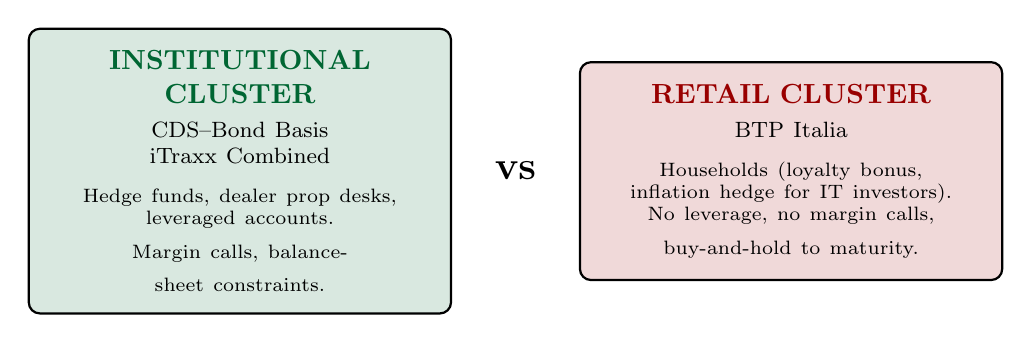
\begin{tikzpicture}
\node[draw, rounded corners, thick, fill=mygreen!15, text width=4.8cm, align=center, inner sep=8pt] (inst) at (-3.5,0) {%
  \textbf{\color{mygreen}INSTITUTIONAL CLUSTER}\\[3pt]
  \footnotesize CDS--Bond Basis\\
  iTraxx Combined\\[6pt]
  \scriptsize Hedge funds, dealer prop desks,\\ leveraged accounts.\\
  Margin calls, balance-sheet constraints.
};
\node[draw, rounded corners, thick, fill=myred!15, text width=4.8cm, align=center, inner sep=8pt] (ret) at (3.5,0) {%
  \textbf{\color{myred}RETAIL CLUSTER}\\[3pt]
  \footnotesize BTP Italia\\[6pt]
  \scriptsize Households (loyalty bonus,\\ inflation hedge for IT investors).\\
  No leverage, no margin calls,\\ buy-and-hold to maturity.
};
\node[font=\Large] at (0,0) {\textbf{vs}};
\end{tikzpicture}

\vspace{0.50cm}

\textbf{Mechanism (\citealp{brunnermeier2009market} + \citealp{vayanos2021preferred}):}
\begin{itemize}\itemsep=0.06cm\footnotesize
  \item \hltb{Institutional cluster:} stress $\rightarrow$ VaR spikes $\rightarrow$ exhaust risk budget
        $\rightarrow$ forced unwinding $\rightarrow$ \emph{both bases widen}.
  \item \hltb{Retail cluster:} insulated from funding shocks $\rightarrow$ behaves as preferred-habitat investors.
\end{itemize}

\vspace{0.30cm}
\centering
\hlt{Natural experiment:} \emph{if co-movement were driven by macro factors, all three would move together.}

\end{frame}

%------------------------------------------------------------------------------
% SLIDE 29 — P1 + P2: Correlations Across Regimes (Two-Cluster Pattern)
%------------------------------------------------------------------------------
\begin{frame}[t]{P1 + P2: Pairwise Correlations Across Stress Regimes}
\centering
\scriptsize
\vspace{0.05cm}

\textit{Pearson correlations of $\Delta m_{i,t}$. LOW $<60$\,bps, HIGH $>120$\,bps iTraxx Main 5Y.}

\vspace{0.25cm}
\renewcommand{\arraystretch}{1.30}
\setlength{\tabcolsep}{8pt}

\begin{tabular}{lcccc}
\toprule
                                  & Uncond.\ & LOW    & MED    & \textit{HIGH} \\
\midrule
\rowcolor{mygreen!15}
CDS--Bond $\leftrightarrow$ iTraxx & $+0.182^{*}$  & $+0.099$ & $+0.098$ & \hlt{$+0.380^{*}$} \\
\midrule
\rowcolor{myred!15}
BTP Italia $\leftrightarrow$ iTraxx & $-0.152^{**}$ & $+0.092$ & $-0.169$ & \hlt{$-0.530$} \\
\rowcolor{myred!15}
BTP Italia $\leftrightarrow$ CDS--Bond & $-0.260^{***}$ & $-0.173$ & $-0.291^{***}$ & \hlt{$-0.345$} \\
\bottomrule
\end{tabular}

\vspace{0.45cm}

\begin{itemize}\itemsep=0.06cm\footnotesize
  \item \textcolor{mygreen}{\textbf{Institutional cluster (P1 + P2 confirmed)}}: CDS--Bond $\leftrightarrow$ iTraxx
        co-moves \emph{positively} and rises monotonically with stress (\hlt{$+0.10 \to +0.38$}).
  \item \textcolor{myred}{\textbf{Sign reversal in retail $\leftrightarrow$ institutional pairs}}:
        BTP Italia $\leftrightarrow$ iTraxx flips from $+0.09$ to \hlt{$-0.53$}; analogous flip vs.\ CDS--Bond.
  \item \hltb{Two-cluster pattern}: positive within institutional, negative across investor-base divide
        $\Rightarrow$ \emph{natural experiment} for Duffie\,(2010).
  \item Robustness: purged correlations, Forbes--Rigobon, DCC-GARCH (backup, App.\ A.8). \textit{Source: Tab.\ 36, Fig.\ 14.}
\end{itemize}

\end{frame}

%------------------------------------------------------------------------------
% SLIDE 29 — P2: Stress Amplification (visual)
%------------------------------------------------------------------------------
\begin{frame}[t]{P2: Stress Amplification --- The Two-Cluster Pattern Visualised}
\vspace{-0.05cm}
\centering

% Figure 14 — regime correlations bar chart
\includegraphics[width=0.70\textwidth,keepaspectratio]{C1_regime_correlations_bar.pdf}

\vspace{0.30cm}

\begin{itemize}\itemsep=0.06cm\small
  \item \emph{Asymmetric amplification under stress.} The institutional cluster
        co-widens; the retail cluster diverges.
  \item \hlt{Critical: not common-macro driven}\,---\,if a single macro factor were responsible,
        all three pairs would amplify in the same direction. They don't.
  \item Investor-base segmentation \emph{is} the experimental treatment.
\end{itemize}

\end{frame}

%------------------------------------------------------------------------------
% SLIDE 30 — P3: Cross-Strategy Spanning + Interaction
%------------------------------------------------------------------------------
\begin{frame}[t]{P3: Cross-Strategy Spanning Regressions}
\centering
\scriptsize
\vspace{0.05cm}

\textit{Following \citet{fleckenstein2014tips}: $\Delta m_{i,t} = \alpha + \sum_{j\neq i}\sum_{l=0}^{2} \beta_{j,l}\,\Delta m_{j,t-l} + \varepsilon_t$.
Newey--West HAC.}

\vspace{0.20cm}

\begin{minipage}[t]{0.46\textwidth}
\centering
\textbf{Cross-strategy spanning $\bar R^2$:}\\[0.10cm]
\renewcommand{\arraystretch}{1.20}
\setlength{\tabcolsep}{6pt}
\begin{tabular}{lc}
\toprule
Dependent: $\Delta m_{i,t}$ & $\bar R^2$ \\
\midrule
CDS--Bond Basis        & 9.7\% \\
\textit{BTP Italia}    & \hlt{13.3\%} \\
iTraxx Combined        & 5.5\% \\
\bottomrule
\end{tabular}\\[0.20cm]
{\footnotesize $\Rightarrow$ \emph{BTP Italia is the most predictable}\,---\,corporate credit cluster has meaningful predictive power for the inflation-linked basis, despite the two-cluster segmentation.}
\end{minipage}\hfill
\begin{minipage}[t]{0.50\textwidth}
\centering
\textbf{Stress interaction (Tab.\ 38):}\\[0.05cm]
{\footnotesize $\Delta m_i = \beta_0\,\Delta m_j + \beta_1(\Delta m_j \times z_t) + \gamma z_t + \varepsilon$}\\[0.15cm]
\renewcommand{\arraystretch}{1.30}
\setlength{\tabcolsep}{4pt}
\begin{tabular}{lc}
\toprule
Pair & $\hat\beta_1$ \\
\midrule
\rowcolor{mygreen!15}
iTraxx $\to$ CDS--Bond  & $+0.186$ (n.s.) \\
\rowcolor{mygreen!15}
CDS--Bond $\to$ iTraxx  & $+0.023$ (n.s.) \\
\midrule
\rowcolor{myred!15}
iTraxx $\to$ BTP Italia & \hlt{$-1.265^{**}$} \\
\rowcolor{myred!15}
BTP Italia $\to$ iTraxx & \hlt{$-0.027^{***}$} \\
\bottomrule
\end{tabular}
\end{minipage}

\vspace{0.30cm}

\begin{itemize}\itemsep=0.04cm\footnotesize
  \item \hlt{Within institutional cluster} (CDS--Bond $\leftrightarrow$ iTraxx): interaction $\beta_1$ positive but \emph{not significant} $\Rightarrow$ co-movement already captured by the linear (non-interactive) effect.
  \item \hlt{Across clusters} (BTP Italia $\leftrightarrow$ iTraxx): interaction $\beta_1$ \emph{strongly negative and significant} (\hlt{$-1.27^{**}$} and $-0.027^{***}$ in the two regression directions) $\Rightarrow$ stress \emph{widens the gap} between the institutional and retail clusters \emph{beyond} what an unconditional correlation would predict. \emph{Source: Tab.\ 38.}
\end{itemize}

\end{frame}

%------------------------------------------------------------------------------
% SLIDE 31 — P3 + P4: VAR — Granger Causality + GIRF
%------------------------------------------------------------------------------
\begin{frame}[t]{P3 + P4: Granger Causality and Liquidity Pecking Order}
\scriptsize
\vspace{0.05cm}

\begin{minipage}[t]{0.40\textwidth}
\centering
\textbf{Granger causality}\\(VAR on $\Delta m_{i,t}$):

\vspace{0.20cm}
\renewcommand{\arraystretch}{1.20}
\setlength{\tabcolsep}{4pt}
\begin{tabular}{lc}
\toprule
Direction & Significance \\
\midrule
iTraxx $\to$ BTP Italia       & \hlt{$1\%$} \\
CDS--Bond $\to$ BTP Italia    & \hlt{$5\%$} \\
\addlinespace
BTP Italia $\to$ iTraxx       & ns \\
BTP Italia $\to$ CDS--Bond    & ns \\
iTraxx $\to$ CDS--Bond        & ns \\
CDS--Bond $\to$ iTraxx        & ns \\
\bottomrule
\end{tabular}\\[0.20cm]
{\footnotesize \emph{Hierarchy:} iTraxx leads $\Rightarrow$ CDS--Bond $\Rightarrow$ BTP Italia, no reverse.}
\end{minipage}\hfill
\begin{minipage}[t]{0.55\textwidth}
\centering
\textbf{GIRF half-lives}\\(\citealp{pesaran1998generalized}):

\vspace{0.10cm}

% Figure 15 — GIRF
\includegraphics[width=0.95\textwidth,keepaspectratio]{E1_girf.pdf}

\vspace{0.10cm}
\renewcommand{\arraystretch}{1.20}
\setlength{\tabcolsep}{8pt}
\begin{tabular}{lc}
\toprule
Strategy & Half-life \\
\midrule
iTraxx Combined        & \hlt{$\sim$2 months} \\
CDS--Bond Basis        & $\sim$4 months \\
\bottomrule
\end{tabular}
\end{minipage}

\vspace{0.20cm}

\begin{itemize}\itemsep=0.04cm\footnotesize
  \item \hlt{P3 hierarchy}: capital arrives first in standardised, exchange-traded index
        $\Rightarrow$ propagates to OTC cash-CDS $\Rightarrow$ finally to retail-dominated inflation-linked.
  \item \hlt{P4 liquidity pecking order}: more liquid $\Rightarrow$ shorter half-life
        (\hlt{iTraxx 2m vs.\ CDS--Bond 4m}).
  \item Cross-response: 1$\sigma$ shock to iTraxx $\Delta m \to$ \emph{negative} response in BTP Italia,
        persists 2--3m $\Rightarrow$ retail-held bonds insulated from funding shock.
\end{itemize}

\end{frame}

%------------------------------------------------------------------------------
% SLIDE 32 — P5: Common Factor → Intermediary Capital
%------------------------------------------------------------------------------
\begin{frame}[t]{P5: Common Factor $\to$ Intermediary Capital, \emph{not} Macro Fundamentals}
\centering
\scriptsize
\vspace{0.05cm}

\textit{First principal component PC1 of the three $\Delta m$ series regressed on intermediary stress
proxies. Newey--West HAC.}

\vspace{0.20cm}
\renewcommand{\arraystretch}{1.20}
\setlength{\tabcolsep}{8pt}

\begin{tabular}{lcc}
\toprule
\textbf{Channel} & \textbf{Proxy} & \textbf{$\hat\beta$ (sign predicted)} \\
\midrule
\multicolumn{3}{l}{\textbf{Panel A. Core proxies (one per channel)}} \\
Intermediary capital   & HKM\_IC \citep{he2017intermediary} & \hlt{$-4.29^{**}$} ($-$ predicted) \\
Funding cost           & LIBOR--OIS spread                  & \hlt{$+3.34^{***}$} ($+$ predicted) \\
Dealer credit risk     & EU prime-broker CDS 5Y             & \hlt{$-0.018^{**}$} ($-$ predicted) \\
Market illiquidity     & Amihud--Mendelson                  & \hlt{$+1.73^{***}$} ($+$ predicted) \\
\addlinespace
\multicolumn{3}{l}{\textit{Model $\bar R^2 = 23.1\%$}} \\
\addlinespace
\multicolumn{3}{l}{\textbf{Panel B. Extended set:} GC-repo--T-bill, EU FCI, settlement fails $\to$ confirms Panel A.} \\
\bottomrule
\end{tabular}

\vspace{0.40cm}

\begin{itemize}\itemsep=0.06cm\footnotesize
  \item \hlt{All four proxies carry the sign predicted by Duffie}: declining intermediary capital,
        rising funding costs, deteriorating dealer credit, and rising market illiquidity all predict
        \emph{wider} mispricings.
  \item \hltb{Common factor is a balance-sheet variable, not a macro fundamental.}
        Direct empirical content of the slow-moving capital theory.
\end{itemize}

\end{frame}

%------------------------------------------------------------------------------
% SLIDE 33 — Why Do These Arbitrages Persist? ★ (chiusura Sezione 5)
%------------------------------------------------------------------------------
\begin{frame}[t]{Why Do These Arbitrages Persist?}
\small

\textbf{A natural question for any paper documenting persistent alpha:
why have these opportunities not been competed away?}

\vspace{0.25cm}

\begin{itemize}\itemsep=0.20cm

  \item \hlt{BTP Italia $\to$ investor-base segmentation.}\ \  Retail holders neither monitor nor
        exploit the relative-value mispricing. Institutional arbitrageurs \emph{can} trade it, but
        the natural counterparty does not unwind in stress
        $\Rightarrow$ \emph{preferred-habitat} bond holder base \citep{vayanos2021preferred}.

  \item \hlt{CDS--Bond $\to$ funding/repo limits.}\ \ Trade requires bond on dealer balance sheet;
        thin EU IG repo market with recall risk; CDS leg consumes regulatory capital
        $\Rightarrow$ \emph{procyclical capacity, countercyclical mispricing}
        \citep{bai2019cds, mitchell2012arbitrage}.

  \item \hlt{iTraxx skew $\to$ post-crisis regulatory capital.}\ \  \citet{boyarchenko2016trends}:
        SLR + Basel III have raised the capital charge for index--single-name basis trades from
        \emph{RoE 6--9\% pre-crisis to 2--3\% post-crisis}.

\end{itemize}

\vspace{0.30cm}

\hltb{Implication.} The mispricings are \emph{not} transient anomalies awaiting competitive
arbitrage\,---\,they are the \emph{equilibrium} outcome of a market in which the cost of intermediary
capital has been \emph{permanently} raised by regulation \citep{mitchell2007slow}.

\end{frame}

%==============================================================================
%  BLOCK 7 — CLOSING  (slides 34-36, ~3 minutes)
%==============================================================================

%------------------------------------------------------------------------------
% SLIDE 34 — Mapping Evidence to Duffie's Five Predictions ★
%------------------------------------------------------------------------------
\section{Closing}

\begin{frame}[t]{All Five Duffie Predictions Find Support}
\scriptsize
\vspace{0.10cm}

\renewcommand{\arraystretch}{1.50}
\setlength{\tabcolsep}{6pt}

\begin{tabular}{p{0.6cm}p{2.8cm}p{8.8cm}p{0.5cm}}
\toprule
\textbf{Pred.} & \textbf{Statement} & \textbf{Empirical evidence} & \\
\midrule
\hlt{P1} & Cross-market correlation
        & Unconditional correlation CDS--Bond $\leftrightarrow$ iTraxx $\Delta m = +0.182^{*}$ (Tab.\ 36).
        & \textcolor{mygreen}{\large\checkmark} \\
\hlt{P2} & Stress amplification
        & Within institutional cluster: $+0.099 \to +0.380^{*}$ (LOW $\to$ HIGH).
          Cross-cluster: $+0.092 \to -0.530$ $\Rightarrow$ \emph{independent evidence of segmentation}.
        & \textcolor{mygreen}{\large\checkmark} \\
\hlt{P3} & Lead-lag transmission
        & Lagged iTraxx $\Delta m$ predicts BTP Italia 1--2m ahead;
          Granger: iTraxx $\to$ BTP Italia at 1\% (Tab.\ 37).
        & \textcolor{mygreen}{\large\checkmark} \\
\hlt{P4} & Liquidity pecking order
        & GIRF half-life: iTraxx $\sim$2m $<$ CDS--Bond $\sim$4m (Fig.\ 15).
        & \textcolor{mygreen}{\large\checkmark} \\
\hlt{P5} & Common factor $=$ intermediary capital
        & PC1 $\to$ HKM ($-4.29^{**}$), LIBOR--OIS ($+3.34^{***}$), Amihud ($+1.73^{***}$), PB CDS ($-0.018^{**}$); $\bar R^2 = 23.1\%$ (Tab.\ 39).
        & \textcolor{mygreen}{\large\checkmark} \\
\bottomrule
\end{tabular}

\vspace{0.45cm}

\centering
\textcolor{myblue}{\textit{``The geography of slow-moving capital is determined not by asset-class labels
but by the network of intermediaries that service these markets\,---\,and ultimately
by who holds the bonds.''}}

\end{frame}

%------------------------------------------------------------------------------
% SLIDE 35 — Summary of Findings
%------------------------------------------------------------------------------
\begin{frame}[t]{Summary of Findings}
\small
\vspace{0.10cm}

\begin{itemize}\itemsep=0.30cm

  \item \hlt{Excess returns are real and robust.}
  Across three benchmark frameworks (Duarte 2007; Brooks 2020; Fung--Hsieh 2004),
  rolling PCA on 85 factors, and AEN with stability selection: positive,
  significant alpha for BTP Italia and CDS--Bond. The iTraxx skew is absorbed by
  its risk factors but emerges as the \emph{leading indicator} of intermediary
  funding stress.

  \item \hlt{Alpha rises systematically in stress.}
  Regime decomposition, Ferson--Schadt conditional alpha, and rolling 36-month
  estimates all point to the same pattern: the unexplained component is
  $2$--$4 \times$ larger when intermediary capital is scarce\,---\,the
  signature of slow-moving capital.

  \item \hlt{Three mispricings linked by an intermediary balance-sheet factor.}
  Two-cluster co-movement (institutional vs.\ retail), liquidity-ordered lead-lag
  (iTraxx $\to$ CDS--Bond $\to$ BTP Italia), and a common PC1 explained by
  intermediary capital, funding cost, and market illiquidity\,---\,not by macro
  fundamentals.

\end{itemize}

\vspace{0.30cm}

\hltb{Bottom line.} Persistent alpha is the \emph{equilibrium} of post-crisis
European credit markets, where regulatory capital costs have permanently raised
the price of intermediary balance-sheet capacity.

\end{frame}

%------------------------------------------------------------------------------
% SLIDE 36 — Limitations & Open Questions
%------------------------------------------------------------------------------
\begin{frame}[t]{Limitations and Open Questions}
\small
\vspace{0.10cm}

\textbf{Three honest limitations of the empirical design:}

\vspace{0.30cm}

\begin{itemize}\itemsep=0.25cm

  \item \hlt{BTP Italia sample begins in March 2012.}\ \  Power constraint on
        regime-dependent tests for this strategy in particular.
        Power for the institutional cluster (samples from 2004 / 2008) is materially stronger.

  \item \hlt{Investor-base segmentation rests on \emph{documented} retail
        dominance of BTP Italia primary market.}\ \  Cross-sectional retail flow not
        observed at instrument level $\Rightarrow$ the preferred-habitat channel is
        \emph{inferred}, not directly tested. A direct test would require holdings
        microdata not yet available to academic researchers.

  \item \hlt{Cross-strategy VAR estimated on the post-2012 sample.}\ \
        Excludes the 2008--09 GFC. But the post-2012 sample \emph{is} the relevant
        regime for intermediary-driven mispricings\,---\,it covers the post-Basel\,III
        ``new normal'' that motivates the regulatory channel of \citet{boyarchenko2016trends}.

\end{itemize}

\vspace{0.30cm}

\hltb{Open question.} Direct testing of the preferred-habitat / retail-flow
channel awaits granular bond-holdings data\,---\,a natural empirical extension as
ECB and Banca d'Italia disclosure regimes evolve.

\end{frame}

%==============================================================================
%  BACKUP SLIDES — for Q&A
%==============================================================================

\section{Backup}

%------------------------------------------------------------------------------
% BACKUP 1 — Full 85-Factor List (placeholder for Table 5)
%------------------------------------------------------------------------------
\begin{frame}[allowframebreaks]{Backup --- Full Factor List (App.\ A.4.1)}
\centering
\footnotesize

% Full factor list — Tab. 5 in paper. Spans multiple slides via allowframebreaks.
% NOTE: Table is long; if it overflows, change frame to [allowframebreaks] or split into panels.
\input{\tablepath/factor_list}

\vspace{0.20cm}

{\footnotesize
Each factor with: name, transformation, frequency, source, reference.
6 panels (Credit / Liquidity \& Funding / Equity \& Intermediary / Volatility / Macro \& Uncertainty / Rates \& Term).}

\end{frame}

%------------------------------------------------------------------------------
% BACKUP 2 — AEN Robustness
%------------------------------------------------------------------------------
\begin{frame}[t]{Backup --- AEN Robustness (App.\ A.6.1)}
\centering
\scriptsize
\vspace{0.10cm}

\textit{Sensitivity to information criterion, adaptive weight exponent $\gamma$,
and pre-cleaning correlation threshold $\rho$.}

\vspace{0.30cm}
\renewcommand{\arraystretch}{1.20}
\setlength{\tabcolsep}{6pt}

\begin{tabular}{lccc}
\toprule
Configuration                     & BTP Italia            & CDS--Bond              & iTraxx Combined \\
\midrule
\textbf{Baseline (HQC, $\gamma=1$, $\rho=0.95$)} & $+1.39^{***}$ & $+3.94^{***}$ & $+0.47$ \\
HQC, $\gamma=0.5$                  & $+1.41^{***}$         & $+3.97^{***}$         & $+0.51$ \\
HQC, $\gamma=2$                    & $+1.37^{***}$         & $+3.92^{***}$         & $+0.43$ \\
HQC, $\rho=0.90$                   & $+1.38^{***}$         & $+3.96^{***}$         & $+0.49$ \\
HQC, $\rho=0.85$                   & $+1.36^{***}$         & $+3.95^{***}$         & $+0.46$ \\
AIC (Friedman default)             & $+1.62^{**}$ (12 fac.) & $+4.28^{***}$ (14 fac.) & $+0.71$ (10 fac.) \\
\bottomrule
\end{tabular}

\vspace{0.40cm}

\begin{itemize}\itemsep=0.06cm\footnotesize
  \item \hlt{Core factor set is identical across configurations.}\ \  Same economic story everywhere.
  \item AIC selects more factors but does not change inference $\Rightarrow$ HQC
        preferred for parsimony.
  \item Stability of selection above $\hat\pi_j \geq 80\%$ threshold for all key factors.
\end{itemize}

\end{frame}

%------------------------------------------------------------------------------
% BACKUP 3 — PCA Robustness
%------------------------------------------------------------------------------
\begin{frame}[t]{Backup --- PCA Robustness (App.\ A.5.1)}
\centering
\scriptsize
\vspace{0.10cm}

\textit{Sensitivity of contemporaneous PCA alpha to window length $W$
and number of components $K$.}

\vspace{0.30cm}
\renewcommand{\arraystretch}{1.20}
\setlength{\tabcolsep}{8pt}

\begin{tabular}{lccc}
\toprule
$(W, K)$               & BTP Italia       & CDS--Bond        & iTraxx Combined \\
\midrule
$(18, 6)$              & $+1.58^{***}$    & $+5.91^{***}$    & $+2.13^{***}$ \\
\textbf{(24, 8) baseline} & $+1.61^{***}$    & $+5.87^{***}$    & $+2.21^{***}$ \\
$(36, 10)$             & $+1.65^{***}$    & $+5.79^{***}$    & $+2.28^{***}$ \\
$(24, 6)$              & $+1.59^{***}$    & $+5.93^{***}$    & $+2.18^{***}$ \\
$(24, 10)$             & $+1.63^{***}$    & $+5.84^{***}$    & $+2.24^{***}$ \\
\bottomrule
\end{tabular}

\vspace{0.40cm}

\begin{itemize}\itemsep=0.06cm\footnotesize
  \item Alpha estimates stable within $\pm 0.10$ p.p.\ across all $(W,K)$ configurations.
  \item Significance unchanged: 1\% in every cell.
  \item Subperiod splits (pre-2012 / 2012--2020 / 2020--2025) confirm stability across regimes.
\end{itemize}

\end{frame}

%------------------------------------------------------------------------------
% BACKUP 4 — Method Comparison Full Table
%------------------------------------------------------------------------------
\begin{frame}[t]{Backup --- Factor Selection Method Comparison (Tab.\ 35)}
\centering
\scriptsize
\vspace{0.10cm}

\renewcommand{\arraystretch}{1.20}
\setlength{\tabcolsep}{5pt}

\begin{tabular}{lcccccc}
\toprule
 & \multicolumn{2}{c}{BTP Italia} & \multicolumn{2}{c}{CDS--Bond} & \multicolumn{2}{c}{iTraxx} \\
\cmidrule(lr){2-3}\cmidrule(lr){4-5}\cmidrule(lr){6-7}
Method                          & $\alpha$        & $k$ & $\alpha$        & $k$ & $\alpha$    & $k$ \\
\midrule
LASSO (HQC)                     & $+1.39^{***}$   & 7  & $+3.91^{***}$   & 11 & $+0.67$     & 13 \\
Elastic Net (HQC)               & $+1.39^{***}$   & 7  & $+3.91^{***}$   & 11 & $+0.67$     & 13 \\
Adaptive LASSO (HQC)            & $+1.39^{***}$   & 7  & $+3.94^{***}$   & 8  & $+0.70$     & 11 \\
\textbf{AEN (HQC, baseline)}    & $+1.39^{***}$   & 6  & $+3.94^{***}$   & 8  & $+0.70$     & 11 \\
ALASSO-Chen (AIC)               & $+0.98$ ($t=1.62$) & 51 & $+4.97^{***}$ & 29 & $+0.74^{*}$ & 19 \\
\bottomrule
\end{tabular}

\vspace{0.40cm}

\begin{itemize}\itemsep=0.06cm\footnotesize
  \item LASSO / EN / Adaptive LASSO converge to the same alpha under HQC tuning.
  \item AEN drops one factor via stability selection ($\hat\Pi_j \geq 0.80$) $\Rightarrow$ \hlt{sparsest, with formal false-selection bound}.
  \item ALASSO-Chen with AIC selects 51 factors for BTP Italia (vs.\ 6 baseline) and \emph{loses} significance ($\alpha = +0.98$, $t = 1.62$) $\Rightarrow$ \hltb{overfitting}: alpha not preserved when the model absorbs noise.
  \item Note: $k$ for iTraxx differs between Tab.\ 33 baseline ($k=5$, $\hat\Pi_j \geq 0.80$) and Tab.\ 35 method comparison ($k=11$, lower threshold for cross-method comparability).
\end{itemize}

\end{frame}

%------------------------------------------------------------------------------
% BACKUP 5 — Subperiod Splits (Benchmark alpha)
%------------------------------------------------------------------------------
\begin{frame}[t]{Backup --- Subperiod Splits (App.\ A.5.2)}
\centering
\scriptsize
\vspace{0.10cm}

\textit{Annualised benchmark alpha across three subperiods (Duarte EUR specification).}

\vspace{0.30cm}
\renewcommand{\arraystretch}{1.20}
\setlength{\tabcolsep}{8pt}

\begin{tabular}{lccc}
\toprule
                       & BTP Italia       & CDS--Bond        & iTraxx Combined \\
\midrule
Pre-2012 (CDS--Bond, iTraxx only) & $-$           & $+5.61^{***}$ & $+3.18^{***}$ \\
2012--2020             & $+1.94^{***}$    & $+4.87^{***}$    & $+3.04^{***}$ \\
2020--2025             & $+2.32^{***}$    & $+5.41^{***}$    & $+4.21^{***}$ \\
\bottomrule
\end{tabular}

\vspace{0.40cm}

\begin{itemize}\itemsep=0.06cm\footnotesize
  \item Significant alpha in \hlt{every subperiod for every strategy}.
  \item Magnitude varies (highest in 2020--2025, COVID + tightening cycle), but the existence of alpha is invariant.
  \item Combined with rolling 36m alpha: alpha is \emph{not} a single-subperiod artefact.
\end{itemize}

\end{frame}

%------------------------------------------------------------------------------
% BACKUP 6 — Purged Correlations + DCC-GARCH + Forbes-Rigobon
%------------------------------------------------------------------------------
\begin{frame}[t]{Backup --- Robustness of Two-Cluster Pattern (App.\ A.8)}
\centering
\scriptsize
\vspace{0.10cm}

\textit{Robustness of regime-correlation findings to alternative methodologies.}

\vspace{0.30cm}
\renewcommand{\arraystretch}{1.30}
\setlength{\tabcolsep}{6pt}

\begin{tabular}{p{4.5cm}p{8.5cm}}
\toprule
\textbf{Methodology}                   & \textbf{Finding} \\
\midrule
\textbf{Raw Pearson} (baseline)        & Two-cluster pattern: $+0.10 \to +0.38$ (institutional);
                                          $+0.09 \to -0.53$ (cross-cluster). \\
\textbf{Purged correlations}           & Residualised on Mkt, SMB, $\Delta$Term, $\Delta$CredSpr.
                                          Two-cluster pattern preserved; magnitudes reduced
                                          by $\sim 10\%$. \\
\textbf{Forbes--Rigobon (2002)}        & Heteroskedasticity-corrected $\rho^*$.
                                          Stress amplification still significant for the institutional cluster;
                                          sign reversal for cross-cluster preserved. \\
\textbf{DCC-GARCH}                     & Time-varying conditional correlations. Same pattern over time:
                                          institutional cluster correlations \emph{rise} during stress episodes
                                          (2008--09, 2011--12, 2020); cross-cluster correlations \emph{fall}. \\
\bottomrule
\end{tabular}

\vspace{0.40cm}

\centering
\hlt{$\Rightarrow$ Two-cluster pattern is structural, not a methodological artefact.}

\end{frame}

%------------------------------------------------------------------------------
% BACKUP 7 — Granger Lag Robustness + Alternative Stress Proxies
%------------------------------------------------------------------------------
\begin{frame}[t]{Backup --- Granger / VAR Robustness (App.\ A.8.3)}
\centering
\scriptsize
\vspace{0.10cm}

\begin{minipage}[t]{0.46\textwidth}
\centering
\textbf{Lag-length robustness (Granger):}\\[0.10cm]
\renewcommand{\arraystretch}{1.20}
\setlength{\tabcolsep}{4pt}
\begin{tabular}{lccc}
\toprule
                               & $p=1$ & $p=2$ & $p=3$ \\
\midrule
iTraxx $\to$ BTP Italia        & $1\%$ & $1\%$ & $5\%$ \\
CDS--Bond $\to$ BTP Italia     & $5\%$ & $5\%$ & $5\%$ \\
BTP Italia $\to$ iTraxx        & ns    & ns    & ns \\
BTP Italia $\to$ CDS--Bond     & ns    & ns    & ns \\
\bottomrule
\end{tabular}
\end{minipage}\hfill
\begin{minipage}[t]{0.50\textwidth}
\centering
\textbf{Alternative stress proxies:}\\[0.10cm]
\renewcommand{\arraystretch}{1.20}
\setlength{\tabcolsep}{4pt}
\begin{tabular}{lc}
\toprule
Stress proxy                            & Pattern preserved? \\
\midrule
iTraxx Main 5Y (baseline)               & \hlt{Yes} \\
iTraxx Crossover                        & Yes \\
V2X (EU equity vol)                     & Yes \\
VIX (US equity vol)                     & Yes \\
HKM intermediary capital ratio          & Yes \\
\bottomrule
\end{tabular}
\end{minipage}

\vspace{0.40cm}

\begin{itemize}\itemsep=0.06cm\footnotesize
  \item Granger transmission hierarchy invariant to lag specification ($p \in \{1,2,3\}$).
  \item Two-cluster co-movement pattern invariant to choice of stress proxy
        $\Rightarrow$ \hlt{not iTraxx-Main-specific}.
\end{itemize}

\end{frame}

%------------------------------------------------------------------------------
% BACKUP 8 — VIF Diagnostics
%------------------------------------------------------------------------------
\begin{frame}[t]{Backup --- VIF Diagnostics (App.\ A.9)}
\centering
\scriptsize
\vspace{0.10cm}

\textit{Variance inflation factors for the three benchmark specifications.}

\vspace{0.30cm}
\renewcommand{\arraystretch}{1.20}
\setlength{\tabcolsep}{6pt}

\begin{tabular}{p{2.5cm}p{4.8cm}p{6.0cm}}
\toprule
Specification              & VIF range          & Notes \\
\midrule
Duarte (2007)              & 1.2--3.5; Fama bond ports R2/R5/R10 $\sim$15--55 & Known correlation in maturity-sorted Treasury portfolios \\
Brooks (2020)              & 1.1--4.8           & All factors $<10$ \\
Fung--Hsieh (2004)         & 1.1--3.2           & All factors $<10$; trend-following uncorrelated \\
\bottomrule
\end{tabular}

\vspace{0.40cm}

\begin{itemize}\itemsep=0.06cm\footnotesize
  \item Two specifications (Brooks, Fung--Hsieh) clean: VIF $<10$ throughout.
  \item Duarte: high VIF only on Fama bond portfolios (well-documented multicollinearity)
        $\Rightarrow$ inference on those coefficients individually is fragile, but the
        \emph{alpha estimate} (intercept) is unaffected.
  \item All AEN-selected factor sets: VIF $<5$ post-stability-selection.
\end{itemize}

\end{frame}

%------------------------------------------------------------------------------
% BACKUP 9 — References (uses \citet{} from main slides)
%------------------------------------------------------------------------------
\begin{frame}[allowframebreaks]{References}
\scriptsize
% references.bib should be in the same folder as this .tex file
\bibliography{references}
\end{frame}

\end{document}